\section{Experiment}

We organized our experiments to answer the following 3 questions: Q1. \textbf{Static Realism \& Stability}: Can the proposed W-DiT structure generate highly realistic and spatiotemporally consistent static environments, especially over extended horizons? Q2. \textbf{Generation Diversity}: Does OccSim exhibit sufficient multimodality and diversity in long-horizon rollout? Q3. \textbf{Dynamic Fidelity \& Downstream Utility}: Can OccSim be used to train temporal-based tasks like 4D semantic occupancy forecasting more effectively than data collected from CARLA?


\subsection{Metrics and datasets}
\label{sec:metrics}

To answer \textbf{Q1}, we assess its performance across two primary dimensions: the realism of the generated static environments and the dynamic fidelity of the traffic simulation. Following previous works \cite{bian2024dynamiccity, yang2025x}, we evaluate static realism via 2D/3D-FID, KID, and MMD (denoted by $\textrm{Dis}$ below).

To formalize realism, we define two evaluation settings to measure the performance of model under different context: \textbf{1. Conditional fidelity}: ${\textrm{Dis}\left( P_{\theta}(\hat{\mathcal{O}}_t | \mathcal{O}_0, J), P_{data}(\mathcal{O}_t | \mathcal{O}_0, J) \right)}$. This evaluates the structural accuracy at each specific time index $t \in \{1, \dots, \mathcal{K}\}$ ($\mathcal{K}$ equal to the length of GT sequence) under the strict constraint of the initial observation $\mathcal{O}_0$ and ego-trajectory $J$. \textbf{2. Unconditional realism}: $\textrm{Dis}\left( P_{\theta}(\hat{\mathcal{O}}_t | \mathcal{O}_0, J), P_{data}(\mathcal{O}) \right)$, where t depend on the rollout length $K$. Although the generation inherently relies on the initial observation $\mathcal{O}_0$ and trajectory $\mathbf{J}$, long-horizon rollouts can reasonably diverge into various valid structures. Therefore, instead of comparing against the strictly paired future frame, we measure the distance between the conditionally generated samples at time $t$ and the global marginal distribution of the entire ground truth training set $\mathcal{O}$. This ensures long-term rollouts universally reside on the valid data manifold.

In \textbf{Q2}, we introduce the Vendi score \cite{friedman2022vendi} and Semantic IoU diverse score. Specifically, the Semantic IoU diverse score evaluates structural divergence in the decoded semantic space by calculating the complement of the average Intersection over Union across multiple stochastic rollouts generated from the same initial scene. Meanwhile, the Vendi score operates in the latent feature space—extracted via a pretrained encoder—to quantify the effective sample size of the generated distributions. These metrics reflect the model's multimodality, where higher scores indicate a richer variety of plausible future layouts, demonstrating the simulator's capability to model environmental uncertainty.

To address \textbf{Q3}, we evaluate the dynamic simulation performance through a zero-shot transfer setting. To the best of our knowledge, we are the first to demonstrate the downstream utility of a data-driven simulator by evaluating its pre-training efficacy on the 4D semantic occupancy forecasting task. Specifically, we utilize continuous data streams collected directly from the ego-vehicle's perspective within our generated simulation. Performance on this downstream task serves as a  proxy, directly reflecting the simulator's capability to faithfully emulate complex, real-world traffic dynamics.

Regarding datasets, we utilize Occ3D-nuScenes \cite{tian2023occ3d} for all static generation realism comparisons to ensure fairness in training data volume. For the remaining experiments, we employ UniOcc-Waymo \cite{wang2025uniocc} or UniOcc-nuScenes due to their unified voxel categorization. Additional simulation metrics and training/implementation details are provided in Appendix~\ref{sec:appendix_training_details}.

\subsection{Main results comparisons}

We first evaluate the realism and stability of the generated static road maps. In Fig. \ref{fig:cond_3d}, we compare our results with previous occupancy world models in terms of both conditional fidelity and unconditional realism. For a comprehensive analysis, our evaluations are conducted across two distinct VAE latent spaces (derived from UniScene \cite{li2025uniscene} and OccFM \cite{liu2025towards}). As illustrated in the figure, our method (shown in red) demonstrates superior long-term stability and structural realism, significantly outperforming baseline models that suffer from rapid error accumulation. Furthermore, due to the limited number of ground truth (GT) samples (fewer than 1000 per timestep $t$), we specifically selected unbiased metrics—namely KID and MMD with two different kernels—to assess conditional fidelity. Here, 1000 frames rollout generated conditioned on straight trajectory after GT's, with constant velocity. 
 
\begin{figure}[htbp]
    \centering
    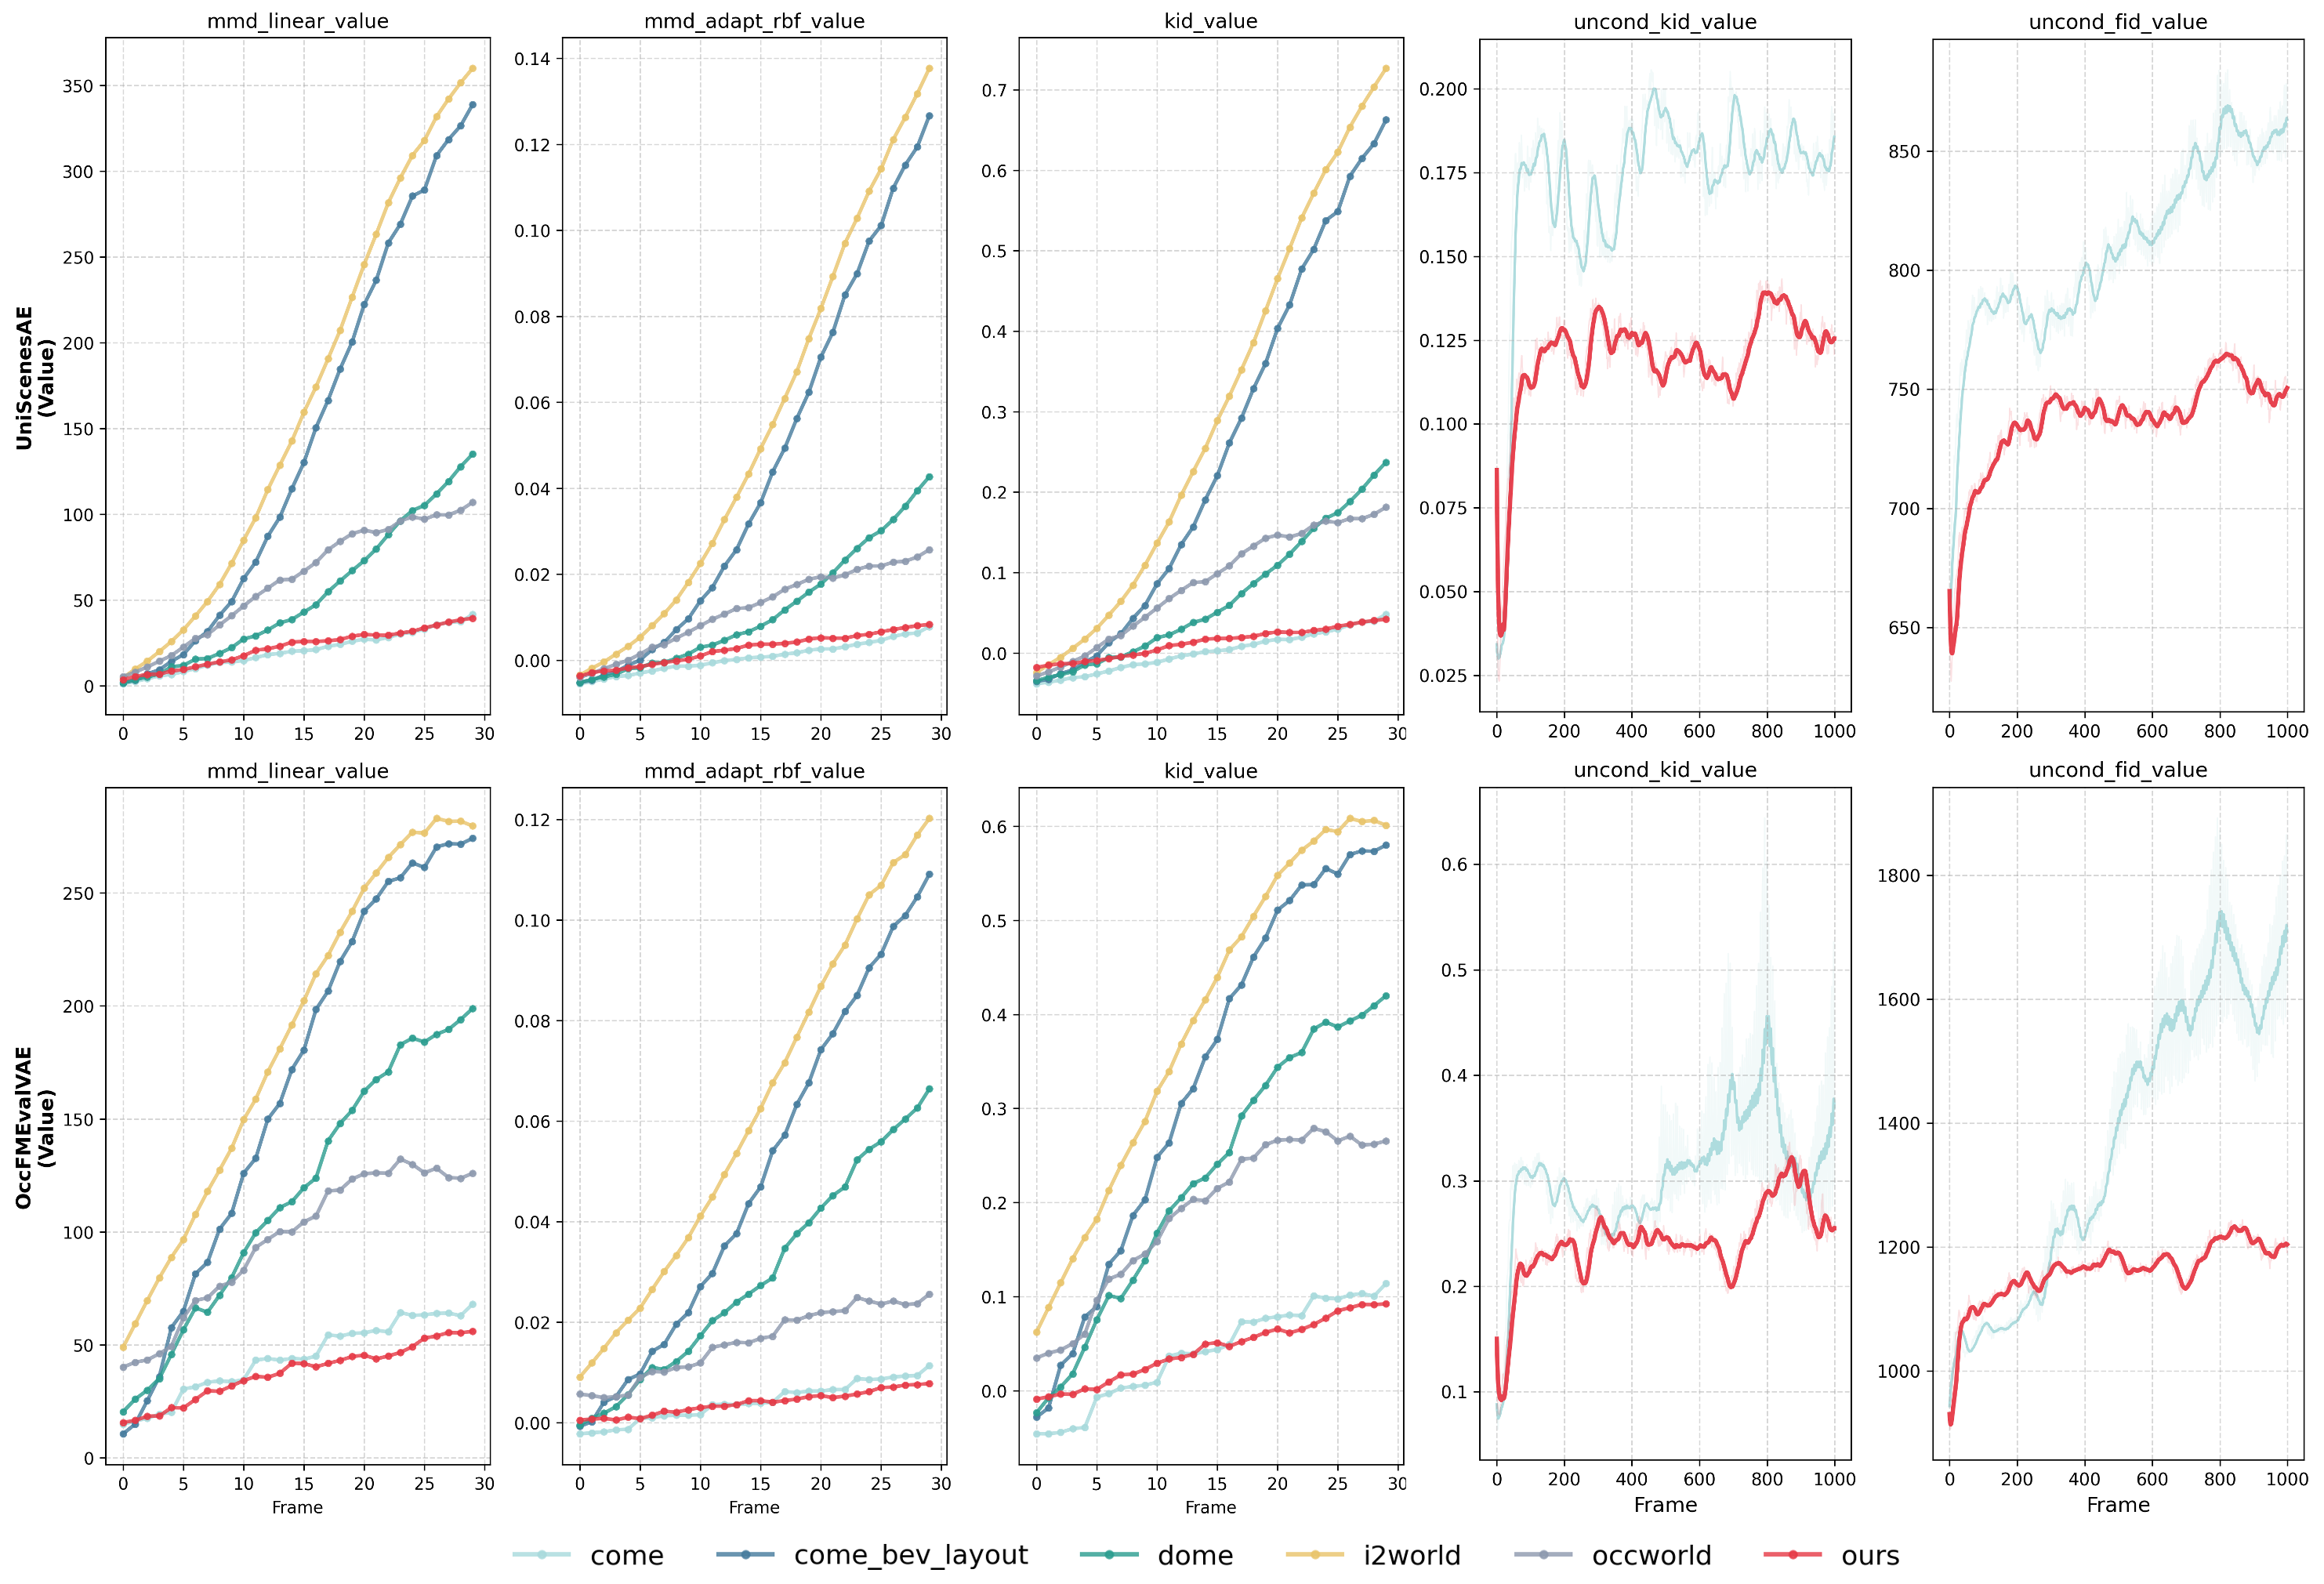
\includegraphics[width=\linewidth]{figures/3d_eval.png}
    \caption{Realism evaluation of generated 3D static occupancy. The left three columns report the conditional fidelity (MMD and KID) under a 30-frame constraint. The right two columns showcase the unconditional realism (KID and FID) over a 1000-frame long-horizon rollout. Our W-DiT-based method obtains the best long-horizon stability and conditional realism.}
    \label{fig:cond_3d}
\end{figure}

This performance gap observed in the 3D occupancy metrics becomes even more pronounced when evaluating realism on the 2D plane. As illustrated in Fig. \ref{fig:uncond_2d}, to increase the rigor of our evaluation, we selected three distinct trajectories to compare our method against the previous state-of-the-art model, COME (details regarding the specific trajectory shapes are provided in Fig.~\ref{fig:traj_vis} of the Appendix). Notably, even when evaluated on the most challenging curved and closed-loop trajectories, our approach still outperforms the previous state-of-the-art method's results on simpler straight-line trajectories.

Furthermore, to establish a lower-bound reference, we constructed a 1000-frame occupancy map collection to serve as a ``chaos'' baseline. This was achieved by randomly selecting structurally collapsed samples from the model's output that lack coherent semantic information. Qualitatively, any metric score surpassing this baseline threshold indicates a completely unusable state. Visualizations of this chaotic baseline collection are available in Appendix~\ref{sec:appendix_chaos}. 

\begin{figure}[t]
    \centering
    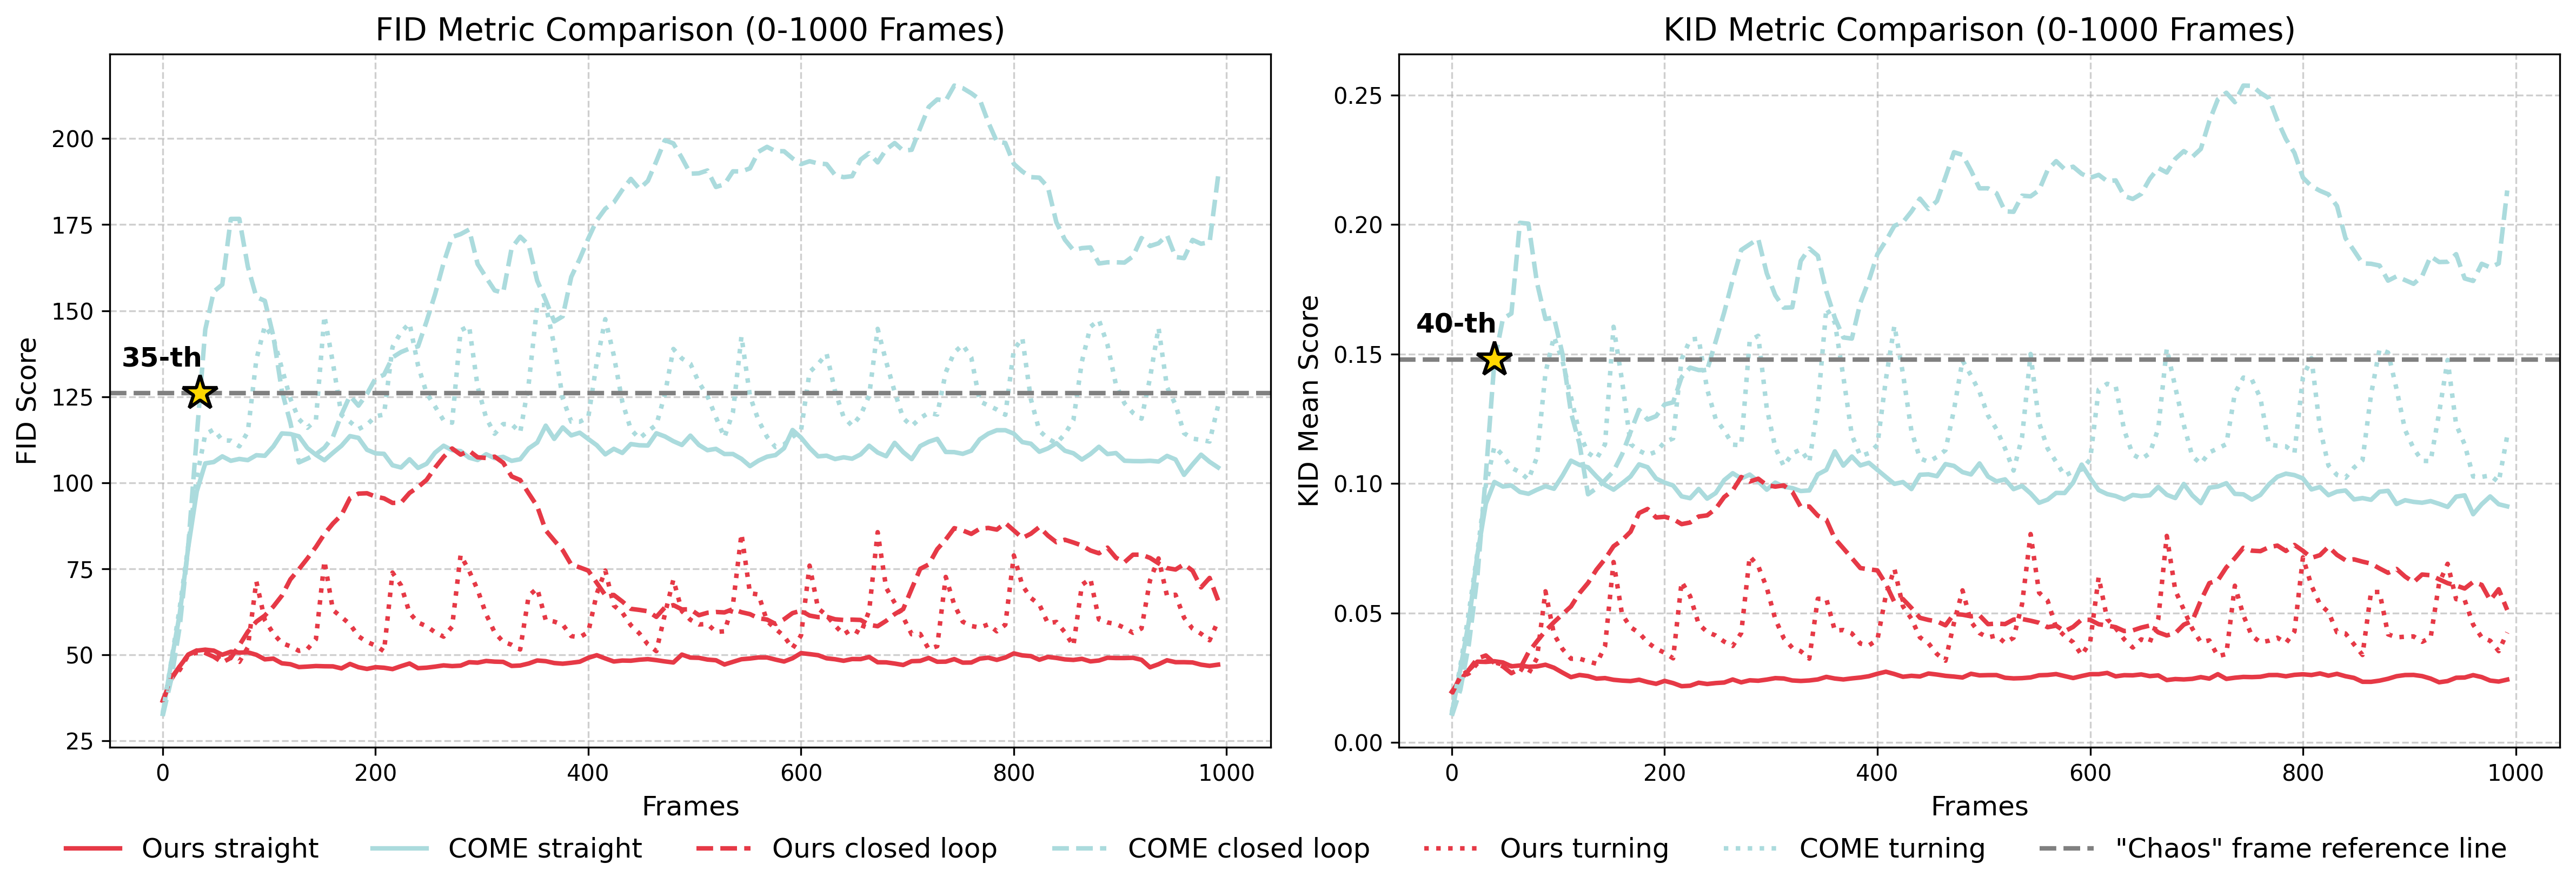
\includegraphics[width=\linewidth]{figures/2dmetrics_comparison.png}
    \caption{Long-horizon 2D realism under varying trajectories. FID and KID comparisons for 2D projections of the 3D generated occupancy. We evaluate three ego-actions: straight, closed-loop, and continuous turning. The dashed reference line indicates the ``chaos'' threshold characterizing scene collapse. In all scenarios, our model (red) remains strictly below this threshold, vastly outperforming the previous SOTA model(which exceed the ``chaos'' threshold in 35/40-th frame generated) and ensuring long-term structural integrity regardless of the driving action. }
    \label{fig:uncond_2d}
\end{figure}

To evaluate the generation diversity over long-term rollouts, we analyze the Pairwise mIoU Diversity and Vendi Scores across first 100 timesteps, as illustrated in Fig. \ref{fig:diversity}. Our proposed method consistently outperforms prior generative baselines. Notably, at early timesteps, our approach demonstrates a rapid increase in diversity, establishing a significant margin over both COME and DOME. As the autoregressive generation extends, our method maintains a high and stable level of diversity without performance degradation. In both OccFM and UniScenes latent spaces, our method achieves the highest Vendi Scores, indicating a richer variety of generated geometric and semantic structures. 

\begin{figure}[h]
    \centering
    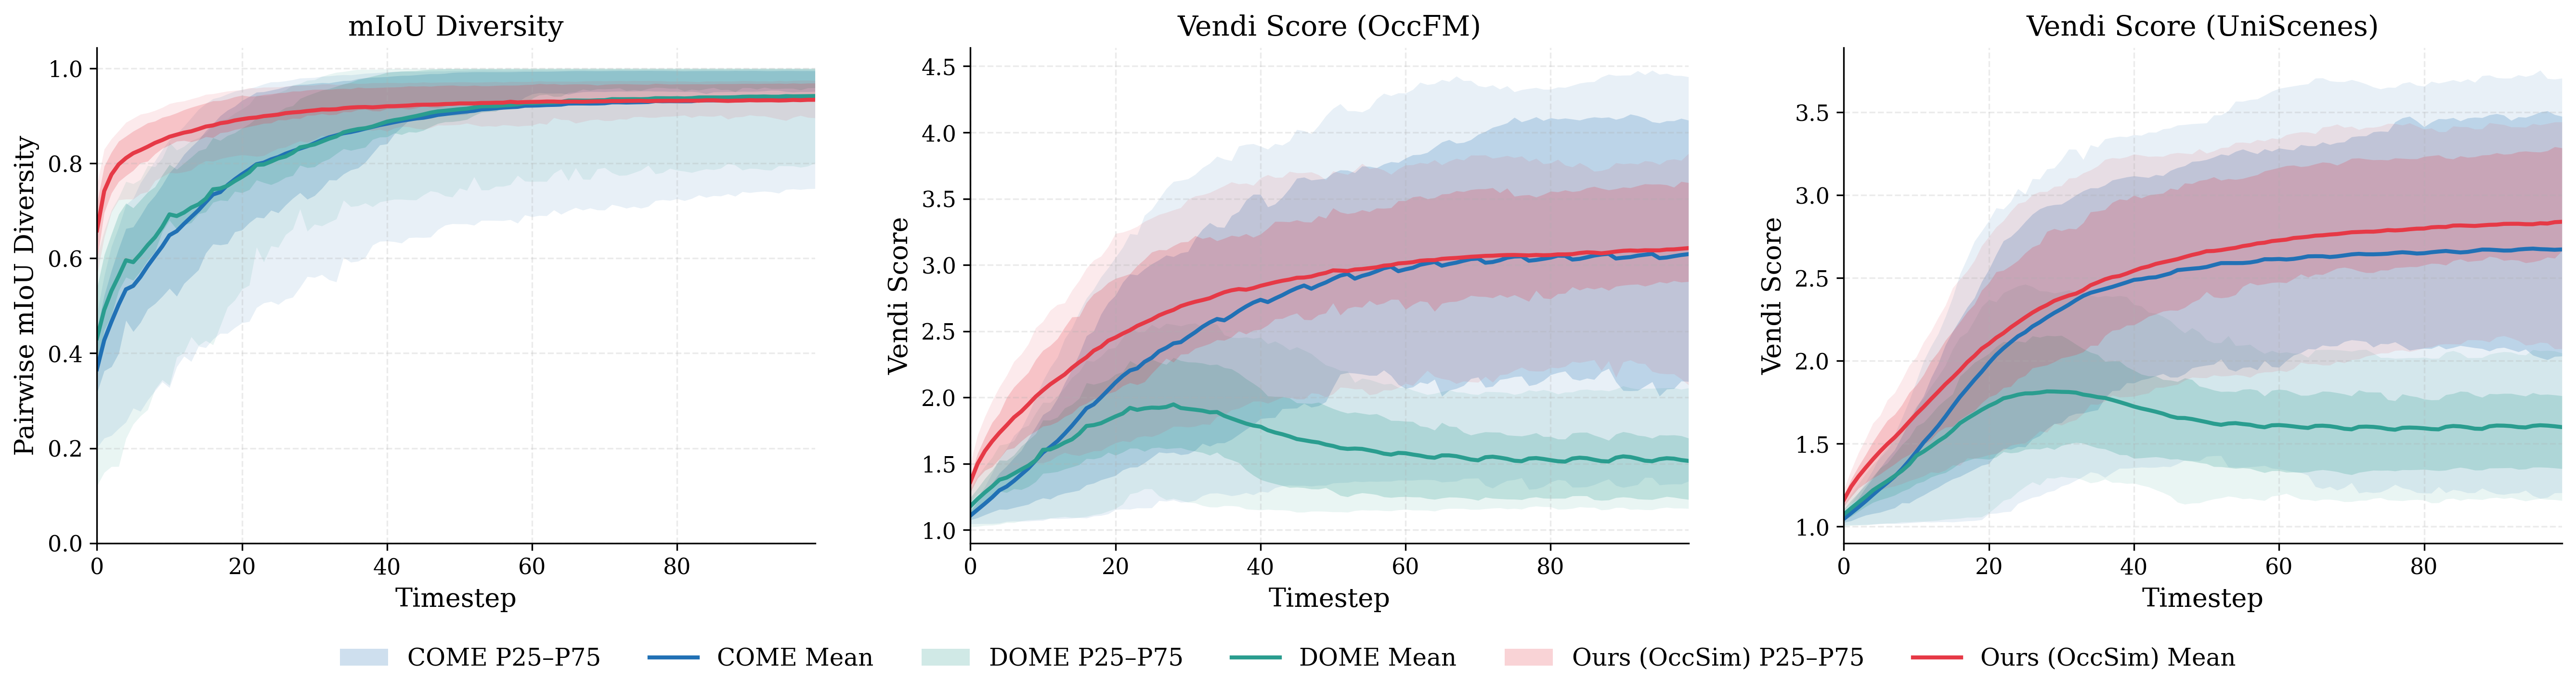
\includegraphics[width=\linewidth]{figures/diversity_combined.png}
    \caption{Generation diversity comparison. Pairwise mIoU diversity and Vendi scores evaluated over 100 timesteps using 10 random seeds. Solid lines and shaded areas denote the mean and the 25th-75th percentiles, respectively. Our methods performed the best diversity in the rollout among all tested generative method.}
    \label{fig:diversity}
\end{figure}

To further validate the practical utility of our generated world, we evaluate OccSim on the downstream task of 4D semantic forecasting. For this experiment, we configure the model to unroll along a curved, closed-loop trajectory, expanding the generation horizon from 1,000 to 3,000 frames to construct a significantly larger map. Based on this extended map, we build the simulation environment utilizing the methodologies detailed in Sec. 3.2 and Sec. 3.3. As demonstrated in Tab. \ref{tab:results_trans}, even when relying on a relatively straightforward dynamics algorithm such as the 2D IDM to control agents, OccSim provides better training signals for simulating overall traffic flow and background dynamics than CARLA. Notably, models trained on data generated by OccSim achieve better performance compared to those trained on the CARLA simulator (Uni-C), showing an improvement of at least $14\%$ relative in average mIoU across the two semantic forecasting models. When we collect 5x more data from UniOcc to train the downstream model, this gap further expands to $52\%$. In terms of 3s average IoU, our method reaches 67\% and 72\% of the upper-bound's performance.

\begin{table}[tb]
  \centering
  \caption{The performance of different semantic forecasting model trained with occupancy collected from UniOcc-Carla(Uni-C) or OccSim, test on UniOcc-NuScenes(Uni-N) validation set. mIOU measured over all background occupancy categories and car category for foreground. $\dagger$: We collected the same amount of data on OccSim as that provided by UniOcc for Carla for fairness. $\star$: Use $\times5$ amount of data collected from OccSim to train downstream models. Stoch.: whether the model is stochastic. The gray-shaded rows represent the performance upper bound, as the models are trained and tested on the same domain without domain shift.}
  \label{tab:results_trans}
    
  \begin{tabularx}{\textwidth}{l lYYYYYYY Y} 
    \toprule
    \multirow{2}{*}{Model} & \multirow{2}{*}{Train Data} & \multicolumn{3}{c}{mIoU} & \multicolumn{3}{c}{IoU} & \multirow{2}{*}{$\text{IoU}_{\text{veh}}$} & \multirow{2}{*}{Stoch.} \\
    \cmidrule(lr){3-5} \cmidrule(lr){6-8}
    &  & 1s & 2s & 3s & 1s & 2s & 3s &  & \\
    \midrule
    \rowcolor{gray!15} OccWorld\cite{zheng2024occworld} & Uni-N & 26.53 & 16.73 & 12.33 & 32.17 & 22.88 & 18.41 & 17.10 & \ding{55} \\
    OccWorld & Uni-C & 11.79 & 8.35 & 6.75 & 18.31 & 14.09 & 12.03 & 6.58 & \ding{55} \\
    $\text{OccWorld}^{\dagger}$ & OccSim & 13.51 & 9.56 & 7.61 & 20.53 & 15.48 & 13.24 & 7.46 & \ding{55} \\
    $\text{OccWorld}^{\star}$ & OccSim & 19.54 & 12.31 & 9.08 & 23.87 & 16.92 & 13.47 & 12.41 &  \ding{55} \\
    \midrule
    \rowcolor{gray!15} OccFM\cite{liu2025towards} & Uni-N & 36.28 & 25.10 & 19.47 & 41.22 & 30.90 & 25.02 & 28.79 & \ding{51} \\
    OccFM & Uni-C & 6.99 & 5.34 & 4.70 & 8.63 & 6.50 & 5.71 & 6.42 & \ding{51} \\
    $\text{OccFM}^{\dagger}$ & OccSim & 15.93 & 11.76 & 9.26 & 18.31 & 14.10 & 11.75 & 13.28 & \ding{51} \\
    $\text{OccFM}^{\star}$ & OccSim & 25.32 & 18.96 & 13.10 & 29.19 & 21.08 & 13.93 & 15.82 & \ding{51} \\
    \bottomrule
  \end{tabularx}
\end{table}


\subsection{Ablation study}
\label{sec:ablation}

In Tab. \ref{tab:ablation}, we conduct a detailed analysis of the perception loss, network architecture, and SNR weighting proposed in our W-DiT design: The success of W-DiT is inextricably linked to these three components. It is evident that without any one of them, achieving stable quality output at the 500-frame scale becomes challenging. Among these, the feature injection structure plays the most significant role. Without this design, the model's output degrades rapidly.

\begin{table}[htbp]
    \centering
    \caption{W-DiT design ablation: we use 3D unconditional realism FID score. When not using the ``local-global'' form of feature aggregation we propose, we directly concatenate the masked condition with the input. The latent here is encoded by AE from UniScenes. }
    \label{tab:ablation}
    \begin{tabular}{ccc | *{7}{p{1.1cm}<{\centering}}} 
        \toprule
        \makecell{Percep.\\Loss} & \makecell{Dual-head\\injection} & \makecell{SNR \\scaled} & 1st & 5th & 10th & 30th & 50th & 100th & 500th\\
        \midrule
        \ding{55} & \ding{55} & \ding{55} & 663.89 & 712.56 & 789.91 & 1023.51 & 1281.99 & 1587.21 & 1612.40 \\
        \ding{55} & \ding{51} & \ding{55} & 637.52  & 708.91  & 924.11 & 992.72 & 1206.50 & 1387.55 & 1672.43\\
        \ding{51} & \ding{51} & \ding{55} & 676.98 & 652.91 & 711.66 & 782.25 & 801.67 & 852.30 & 901.57 \\
        \ding{51} & \ding{51} & \ding{51} & 665.23 & 630.34 & 645.96 & 687.90 & 698.87 & 712.65 & 744.71 \\
        \bottomrule
    \end{tabular}
\end{table}
